\section{Lógica de las Instancias de Retrofit}

La aplicación móvil se comunica con los servicios backend a través de Retrofit, una biblioteca de cliente HTTP de tipo seguro para Android y Java. Retrofit simplifica enormemente el proceso de realizar solicitudes de red, mapeando APIs RESTful a interfaces Kotlin con anotaciones. Para gestionar la interacción con los distintos servidores, el sistema utiliza dos instancias de Retrofit, cada una configurada específicamente para su respectivo servicio.

\subsection{Configuración de Instancias de Retrofit}

Ambas instancias de Retrofit utilizan `GsonConverterFactory` para la serialización y deserialización de objetos JSON, y `OkHttpClient` para la gestión de las operaciones HTTP subyacentes, incluyendo la configuración de timeouts.

\subsubsection{Instancia para el Servidor Java Spring-Boot}

Esta instancia de Retrofit está dedicada a la comunicación con el servidor principal de lógica de negocio, el Servidor Java Spring-Boot, desplegado en Azure. Su configuración prioriza la fiabilidad y un balance adecuado en los tiempos de respuesta para las operaciones transaccionales.

\begin{itemize}
	\item \textbf{`RetrofitInstance` (Objeto Singleton):} Implementado como un objeto singleton para asegurar que solo exista una única instancia de Retrofit para este servidor en toda la aplicación, optimizando recursos.
	\item \textbf{`OkHttpClient`:} Se utiliza un cliente HTTP personalizado con los siguientes timeouts:
	\begin{itemize}
		\item `connectTimeout(10, TimeUnit.SECONDS)`: Establece un tiempo máximo de 10 segundos para establecer una conexión con el servidor.
		\item `writeTimeout(120, TimeUnit.SECONDS)`: Permite hasta 120 segundos para enviar un cuerpo de solicitud al servidor.
		\item `readTimeout(120, TimeUnit.SECONDS)`: Define un límite de 120 segundos para recibir una respuesta completa del servidor.
	\end{itemize}
	Estos tiempos están ajustados para manejar operaciones que podrían requerir un procesamiento moderado en el servidor, sin ser excesivamente laxos.
	\item \textbf{`GsonConverterFactory.create()`:} Utilizado para convertir automáticamente objetos Kotlin en JSON para las solicitudes y viceversa para las respuestas.
\end{itemize}
Esta configuración asegura una comunicación eficiente y tolerante a cierto nivel de latencia con el servidor principal de la aplicación.

\begin{figure}[htbp!]
	\begin{center}
		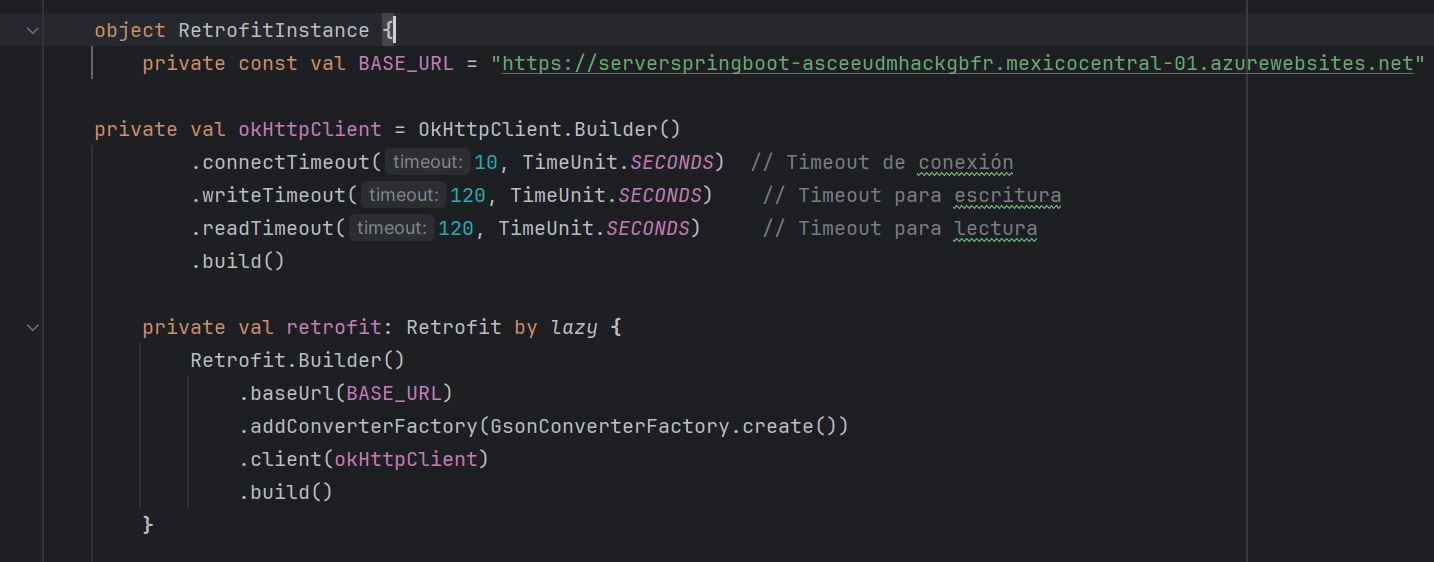
\includegraphics[width=0.9\textwidth]{ImagenesDetalles/Retrofit1}
		\caption{RetrofitCamaraInstance.}
		\label{fig:DetallesRetrofit1}
	\end{center}
\end{figure}

\subsubsection{Instancia para el Servidor de la Red Neuronal}

Esta instancia de Retrofit está optimizada para interactuar con el **Servidor Red Neuronal**, también alojado en Azure, que es responsable específicamente de las funcionalidades de reconocimiento facial. Dada la naturaleza de estas operaciones (envío de imágenes y procesamiento intensivo), se requieren timeouts más generosos.

\begin{itemize}
	\item \textbf{`RetrofitCamaraInstance` (Objeto Singleton):} Similar al anterior, es un singleton para una gestión eficiente de la conexión con el servidor de la red neuronal.
	\item \textbf{`OkHttpClient` con `HttpLoggingInterceptor`:}
	\begin{itemize}
		\item `HttpLoggingInterceptor().apply { level = HttpLoggingInterceptor.Level.BODY }`: Se incluye un interceptor de logging para fines de depuración y monitoreo. Este interceptor permite registrar en detalle (cuerpo incluido) las solicitudes y respuestas HTTP, lo cual es invaluable durante el desarrollo y la fase de pruebas para entender el flujo de datos.
		\item `connectTimeout(300, TimeUnit.SECONDS)`: Configurado a 300 segundos (5 minutos) para permitir conexiones en entornos con latencia o carga.
		\item `writeTimeout(300, TimeUnit.SECONDS)`: Permite hasta 300 segundos para la escritura de datos, esencial para el envío de imágenes que pueden ser de tamaño considerable.
		\item `readTimeout(300, TimeUnit.SECONDS)`: Un timeout de lectura de 300 segundos para esperar la respuesta del servidor, anticipando que el procesamiento de la red neuronal puede ser intensivo y tomar tiempo.
	\end{itemize}
	\item \textbf{`GsonConverterFactory.create()`:} También utilizado para la serialización/deserialización JSON.
\end{itemize}
La configuración de esta instancia subraya la necesidad de manejar operaciones que implican el envío de datos más pesados (imágenes) y un procesamiento que puede ser más lento, asegurando que la conexión no se cierre prematuramente.

\begin{figure}[htbp!]
	\begin{center}
		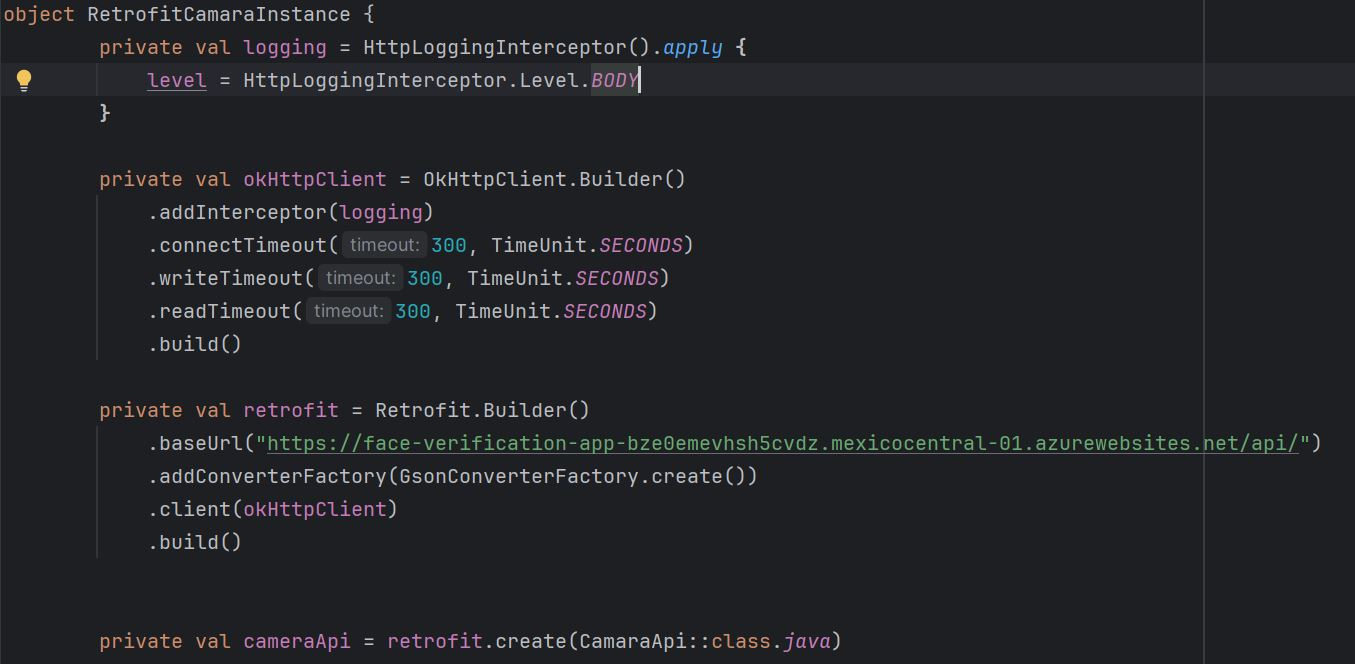
\includegraphics[width=0.9\textwidth]{ImagenesDetalles/Retrofit2}
		\caption{RetrofitCamaraInstance.}
		\label{fig:DetallesRetrofit2}
	\end{center}
\end{figure}

